%%%%%%%%%%%%%%%%%%%%%%%%
%
% $Autor: Wings $
% $Datum: 2020-07-24 09:05:07Z $
% $Pfad: GDV/Vortraege/latex - Ausarbeitung/Kapitel/Bezier.tex $
% $Version: 4732 $
%
%%%%%%%%%%%%%%%%%%%%%%%%

\section{Allgemeine mathematische Beschreibung Bézier-Kurve}

Bézier curves are formed with the help of Bernstein polynomials. If at least two points and two tangents are known, control points can be determined with which a control polygon is formed. The course of the curve is oriented to this control polygon. The number of control points depends on the degree of the Bézier curve.  A Bézier curve of degree n has n+1 control points.  The Bézier curve is calculated using the De Casteljau algorithm.

\bigskip

\DEF
{
  In the interval $[0;\, 1]$ the \textbf{ Bernstein polynomial of n\textsuperscript{th} degree} is defined by:
	
  \begin{equation}
	b_{i,n}(\lambda) = \binom{n}{i} (1-\lambda)^{n-i} \lambda^{i}, \quad \lambda \in [0,1], \quad i=0,\dots,n
	\label{Bernsteinpolynome}
  \end{equation}
}

\bigskip

\DEF
{
  The binomial coefficient is defined by:
    
 \begin{equation}
   \binom{n}{i}=\frac{n!}{i!(n-i)!}, \quad i=0, \dots ,n  
   \label{Binomialkoeffizient}
 \end{equation}
}	

\bigskip

Here the Bernstein polynomials $b_{i,n}$ form a basis of the vector space $\Po^n(I)$ of polynomials of degree at most $n$ over $I$. Thus every polynomial of degree at most $n$ can be written uniquely as a linear combination.	%P in mathematical 
\cite{Farin:2002}

\bigskip

\BEISPIEL{
  Determination of Bernstein polynomials for $n = 3 $ holds:

  $$
    \begin{array}{*4{>{\displaystyle}c}}
      b_{3,0}(\lambda) &= \binom{3}{0} (1-\lambda)^{3-0} \lambda^{0} &=& (1-\lambda)^{3}\\  \\
      b_{3,1}(\lambda) &= \binom{3}{1} (1-\lambda)^{3-1} \lambda^{1} &=& 3\lambda(1-\lambda)^{2} \\  \\
      b_{3,2}(\lambda) &= \binom{3}{2} (1-\lambda)^{3-2} \lambda^{2} &=& 3\lambda^2(1-\lambda)\\ \\
      b_{3,3}(\lambda) &= \binom{3}{3} (1-\lambda)^{3-3} \lambda^{3} &=& \lambda^3 
    \end{array}
  $$

  $b_{3,i}(\lambda)$ with $i=0, 1, 2, 3$ are the cubic Bernstein polynomials of degree 3.
}	

\bigskip

\begin{figure}
  \begin{center}
   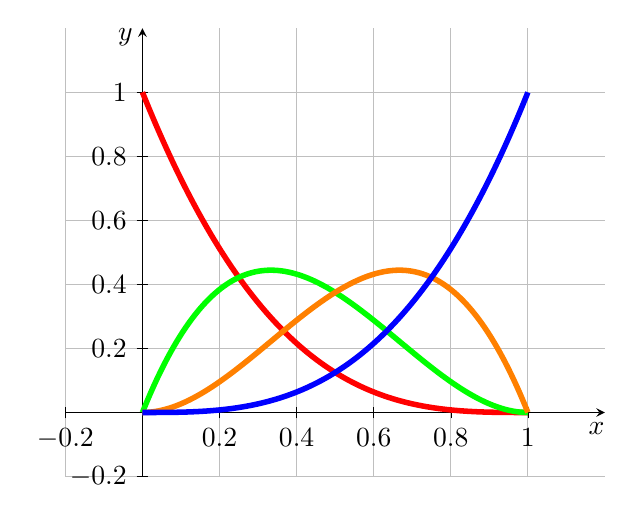
\begin{tikzpicture}[scale=1.0,
   declare function={  B30(\x)   =pow(1-\x,3); 
                       B31(\x)   =3*\x*pow(1-\x,2);
                       B32(\x)   =3*\x*\x*pow(1-\x,1);
                       B33(\x)   =pow(\x,3); 
                    },domain=0:1,smooth]
  \begin{axis}[
%      width=6cm,height=6cm,
      axis lines=middle,
      domain=0:1,
      smooth,
      no markers,
      grid,
      xmin=-0.2,xmax=1.2,
      tick style=black,
      xtick={-0.2,0,...,1},
      xlabel=$x$,
      xlabel style={below, anchor=north east,inner xsep=0pt},
      restrict y to domain=0:1,
      ymin=-0.2,ymax=1.2,
      ytick={-0.2,0,...,1},
      ylabel=$y$,
      ylabel style={above,anchor=north east,inner ysep=0pt},
      samples=100,
    ]
    \addplot[red,line width=2pt]{B30(\x)};
    \addplot[green,line width=2pt]{B31(\x)};
    \addplot[orange,line width=2pt]{B32(\x)};
    \addplot[blue,line width=2pt]{B33(\x)};
  \end{axis}

    \end{tikzpicture} 
  \caption{Bernstein polynomial of degree $3$}
  \end{center}
\end{figure}

\bigskip

\DEF{
  Given are the points 

  $$
	Q_{i} =	\left(
	\begin{array}{c}
	x_{i} \\
	y_{i}
	\end{array}
	\right) \quad \hbox{mit} \quad Q_{i} \in \R^2, \quad i = 0, 1, \ldots, n
  $$	
	
  A \textbf{Bézier curve} is then defined by
	
  \begin{equation}
	C(\lambda) = \sum_{i=0}^n Q_{i}\cdot  b_{i,n}(\lambda)
	\label{Bezierkurve}
  \end{equation}
	
  The points $Q_i, i=0, \ldots, n$ are called \textbf{control points}.	
}	
	
\bigskip

The control points of a Bézier curve form the so-called control polygon.

\bigskip

\Bemerkung{
  Let the starting point $P_0$ and the end point $P_1$, as well as the tangents $\vec{t}_0$ and $\vec{t}_1$ be given. The tangents are not necessarily normalised.

  The control points $Q_{0},Q_{1}, Q_{2}$ and $Q_{3}$ of the associated Bézier curve are given by the following equations:

  \begin{equation}
    Q_{0}=P_{0},
    \qquad    
    Q_{1}=P_{0}+\lambda_{0} \vec{t}_{0},  
    \qquad   
    Q_{2}=P_{1}-\lambda_{1} \vec{t}_{n}, 
    \qquad    
    Q_{3}=P_{1}
	\label{KPunkte4}
  \end{equation}

  \cite{Jaklic:2010}	
}



\bigskip

\BEISPIEL{ \label{KPunkte4Beispiel}
  Given are
  $$
    P_0 = \binom{2}{4}, 
    \quad
    \vec{t}_0 = \binom{1}{1}
    \quad \hbox{und} \quad 
    P_1 = \binom{6}{1},
    \quad
    \vec{t}_1= \binom{1}{-2}
  $$    
  
  Then, according to theorem \ref{Kpoints4} for control points of the associated Bézier curve results:
  
  $$
    Q_{0}=P_{0} = \binom{2}{4},
    \qquad    
    Q_{1}=P_{0}+\vec{t}_{0}
     = \binom{2}{4}+\binom{1}{1}=\binom{3}{5},  
  $$
  
  $$  
    Q_{2}=P_{1}- \vec{t}_{n}
         = \binom{6}{1} -\binom{1}{-2} = \binom{5}{3} , 
    \qquad    
    Q_{3}=P_{1} = \binom{6}{1}
  $$
 
  The Bézier curve and its control points are shown in the figure \ref{KPoints4Graph}. 
}
  
\begin{figure}
  \begin{center}
   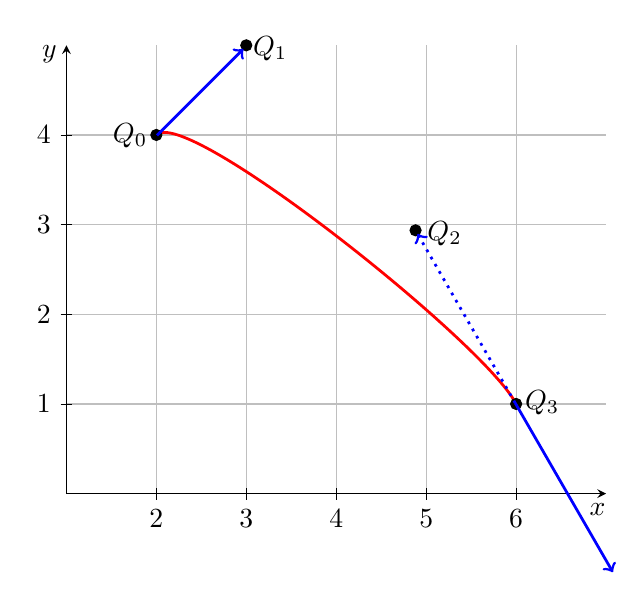
\begin{tikzpicture}[scale=1.0,
   declare function={  FX(\x)   =-6*pow(\x,3)+9*pow(\x,2)+\x+2; 
                       FY(\x)   = 5*pow(\x,3)-9*pow(\x,2)+\x+4; 
                    },domain=0:1,smooth]
  \begin{axis}[
%      width=6cm,height=6cm,
      axis lines=middle,
      domain=0:1,
      smooth,
      no markers,
      grid,
      xmin=1,xmax=7,
      tick style=black,
      xtick={1,2,...,6},
      xlabel=$x$,
      xlabel style={below, anchor=north east,inner xsep=0pt},
      restrict y to domain=-12:12,
      ymin=0,ymax=5,
      ytick={0,1,...,4},
      ylabel=$y$,
      ylabel style={above,anchor=north east,inner ysep=0pt},
      samples=100,
    ]
    \addplot[red,line width=1.0pt] ({FX(\x)}, {FY(\x)});
    \addplot[color = black,
    fill  = black,only marks] plot coordinates {(2,4) (6,1)
    ({2+1.414*cos(45)},{4.+1.414*sin(45)})
    ({6-2.236*cos(-60)},{1-2.236*sin(-60)}) };
    
    
  \end{axis}

    \coordinate[label=left:$Q_0$]  (P0) at (1.15,4.55);
    \coordinate[label=right:$Q_3$]  (P1) at (5.7,1.15);

    \coordinate[label=right:$Q_1$]  (P0T) at ({1.15+1.55*cos(45)},{4.55+1.55*sin(45)});
    \coordinate  (P1T) at ({5.7+2.48*cos(-60)},{1.15+2.48*sin(-60)});
    \coordinate[label=right:$Q_2$]  (P1Tn) at ({5.7-2.48*cos(-60)},{1.15-2.48*sin(-60)});
    
    \draw [blue,line width=1.0pt,->] (P0) -- (P0T);
    \draw [blue,line width=1.0pt,->] (P1) -- (P1T);
    \draw [blue,line width=1.0pt,->,dotted] (P1) -- (P1Tn);

    

    \end{tikzpicture} 
  \end{center}
  \caption{Bézier curve for example \ref{KPunkte4Beispiel} }
  \label{KPunkte4Graph}
\end{figure}
